% 6. Results
%   6.1. Anatomical
%   6.2. Mechanical Simulation
\section{Results}
\label{sec:results}

% - Disegno surrogato anatomico dell'albero respiratorio.  (output da
%   ParaView).
% - Grafici: un gradino "sopra" (10) le soglie e uno "sotto" (8) (xlims
%   = (.995, 1.09)).

% Grafici dipendenti dal numero di generazioni (?)

\subsection{Anatomical}
\label{subsec:anatomical_results}

% AGGIUNTA MODIFICA, COMPLETARE
A CT of a 40 week infant was collected. We segmented and extracted the
centreline of XX airways , down to XX generation.  We also obtained
four lobes.
% Mostra immagine delle vie aeree segmentate (skeletonizzazione della
% centreline) e dei quattro lobi su tre piani (xy, xz, yz).

\begin{figure}[H]\centering
  \subfloat[][x-y plane]{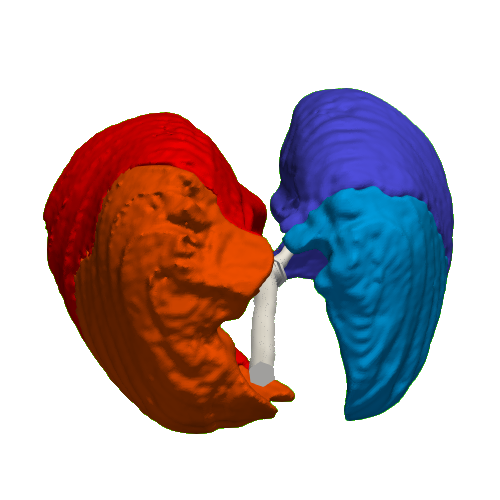
\includegraphics[width=.45\textwidth]{major_airways_xy.png}}%
  \hspace{1cm}
  \subfloat[][y-z plane]{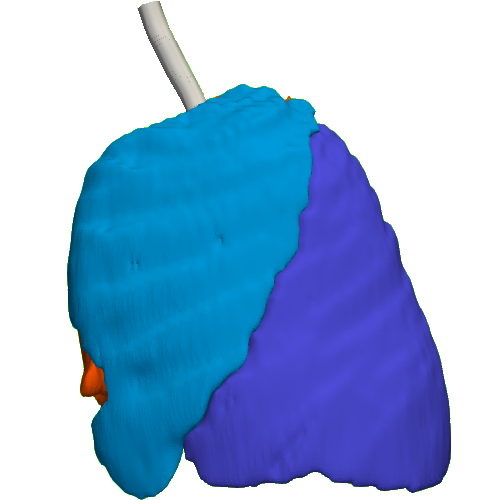
\includegraphics[width=.45\textwidth]{major_airways_yz.png}}\\
  \subfloat[][x-z plane]{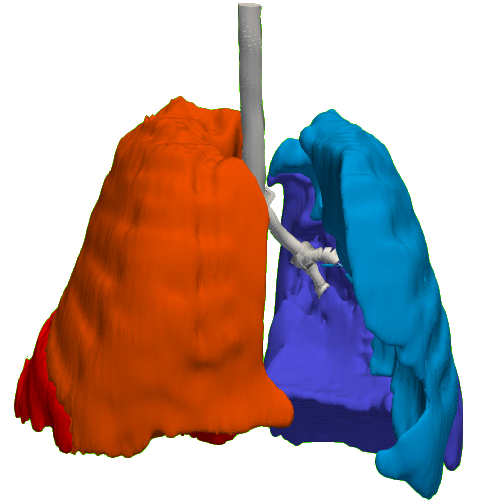
\includegraphics[width=.45\textwidth]{major_airways_xz.png}}

  \caption{Major Airways and Lobes segmentations.  Cyan: Upper Left
    Lung; Blue: Lower Left Lung; Orange: Upper Right Lung; Red: Lower
    Right Lung.}
  \label{fig:anatomical_results}
\end{figure}

Using the developed program, based on Lung Chaste library, we managed
to reconstruct the missing generations. The lowest generation was
XX. The obtained airway tree can be displayed by ParaView.
% Mostra immagine dell'albero completo.

\begin{figure}[H]\centering
  \subfloat[][x-y plane]{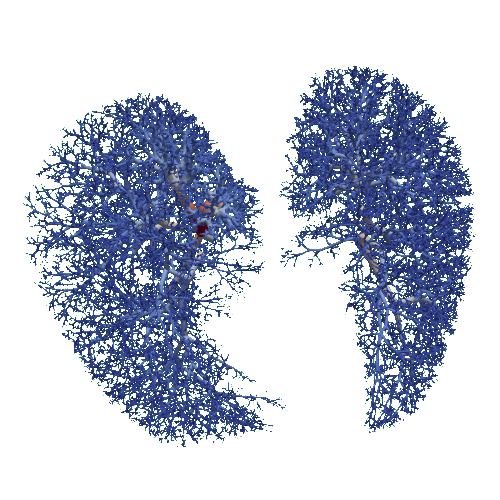
\includegraphics[width=.45\textwidth]{complete_airways_xy.png}}%
  \hspace{1cm}
  \subfloat[][y-z plane]{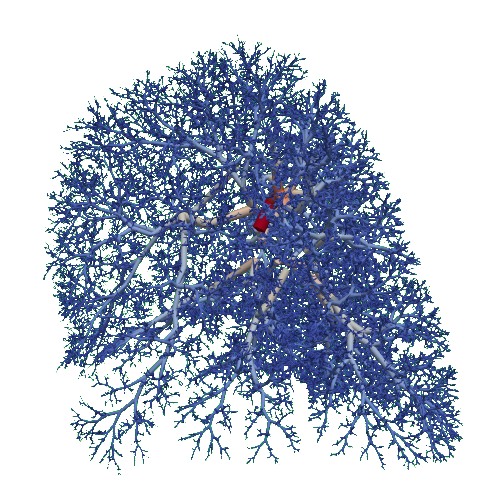
\includegraphics[width=.45\textwidth]{complete_airways_yz.png}}\\
  \subfloat[][x-z plane]{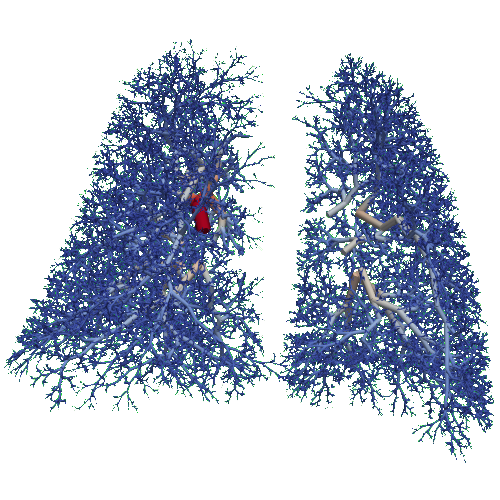
\includegraphics[width=.45\textwidth]{complete_airways_xz.png}}

  \caption{Complete Airways generated by Chaste User Project (major
    airways are here excluded).  They are colorcoded with respect to
    their radii.}
  \label{fig:complete_anatomical_results}
\end{figure}

The lobes are fully covered by the statistically-generated airways and
this allows to move a step forward in newborn lung simulation.

\subsection{Mechanical Simulation}
\label{subsec:mechanical_results}

% Descrizione dei test.  La descrizione della rete in termini di
% parametri va fatta qui?

% Introduzione da aggiungere: lo scopo di queste simulazioni. Queste non
% sono le simulazioni per capire come va il bambino ma per verificare la
% coerenza dei comportamenti dei vari componenti.  Facendo riferimento
% alla figura della sottorete che ho considerato.  Nella sottorete
% abbiamo applicato due livelli diversi di pressione: una sopra la
% pressione capillare, così da aprire tutti i diodi dei vari moduli e
% una sotto la pressione capillare di qualche diodo per vedere le
% differenze.

These simulations are to verify the various components and modules
coherence.  This model is still very far from its conceived
application in a clinical context.  Two tests have been designed as
follows.  A step voltage generator is applied to the electrical
equivalent of the newborn lung.  The step amplitude is 10V for the
first test, 8V for the second one.

The reason why these values for voltage have been chosen are related
both to the airway subtree described in \Cref{fig:subtree_development}
and to the diode threshold values ``vin\_th'' for airways and acini in
\Cref{tab:airways_test1,tab:acini_test1,tab:airways_test2,tab:acini_test2}.

% Faccio una descrizione di queste curve: si aprono le vie aeree dalla
% più vicina a quella più lontana e gli acini seguono un determinato
% ordine di apertura.

% Quando cambio soglia abbiamo notato che alcuni acini non si aprono
% in quanto la pressione capillare è troppo elevata.  Il fatto di aver
% abbassato la pressione ha rallentato l'apertura di tutti quanti perché
% ci mettono un po' a raggiungere la pressione capillare.  Cambia la
% sequenza di apertura degli acini.  Posso usare nella descrizione dei
% grafici anche i nomi IAE, IAI ecc (facendo però riferimento al
% capitolo in cui introduco il problema).

% AGGIUNTA MODIFICA, COMPLETARE
% In order to verify the behavour of the mechanical components
% implemented in Julia, we tested the system described in by applying

The first test employs a step amplitude for voltage generator which
ovecomes every module diode threshold.  It is possible to check-out in
\Cref{fig:mechanical_results_10,fig:mechanical_results_8} modules
opening times and activation orders.  Airways open from the most
proximal to the most distal one.  It is more interesting to analyze
the activation order of the acini.  They open following a proximal
to distal order but high diode thresholds introduce delays.

% Inserisco gli output di Julia, in particolare correnti e tensioni
% sotto e sopra threshold. (ampiezza scalino di 8 e 10V).

\begin{figure}[H]\centering
  \subfloat[][Airways voltages]{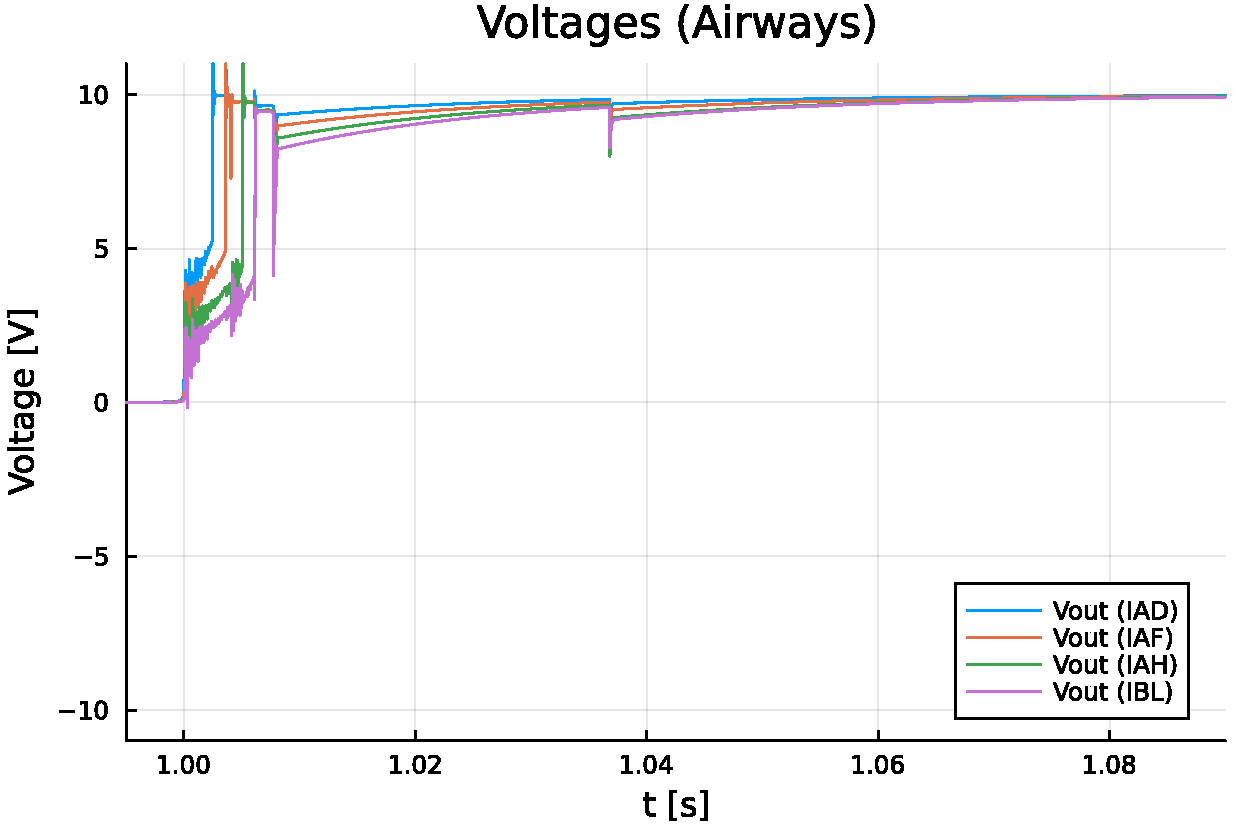
\includegraphics[height=.20\textheight]{airways_voltages_10.pdf}}%
  \hspace{1cm}
  \subfloat[][Airways currents]{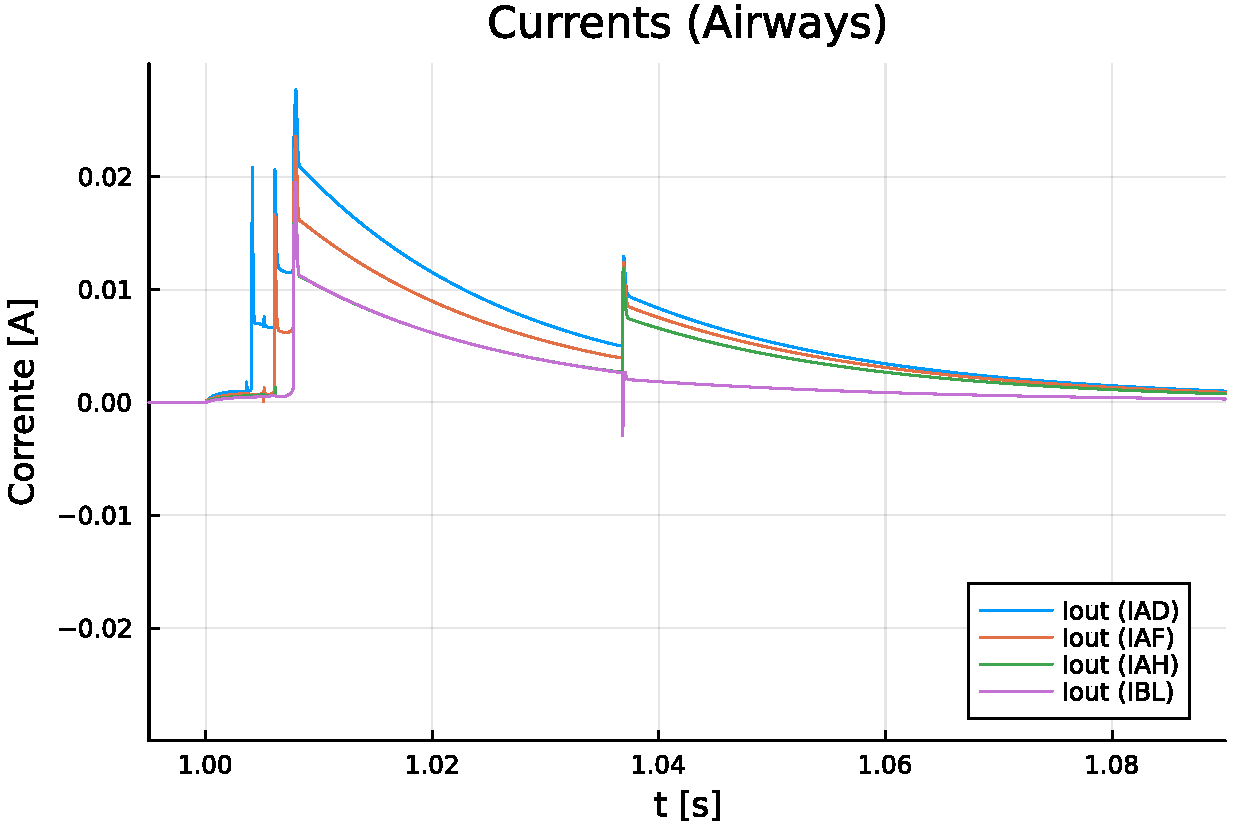
\includegraphics[height=.20\textheight]{airways_currents_10.pdf}}\\
  \subfloat[][Acini voltages]{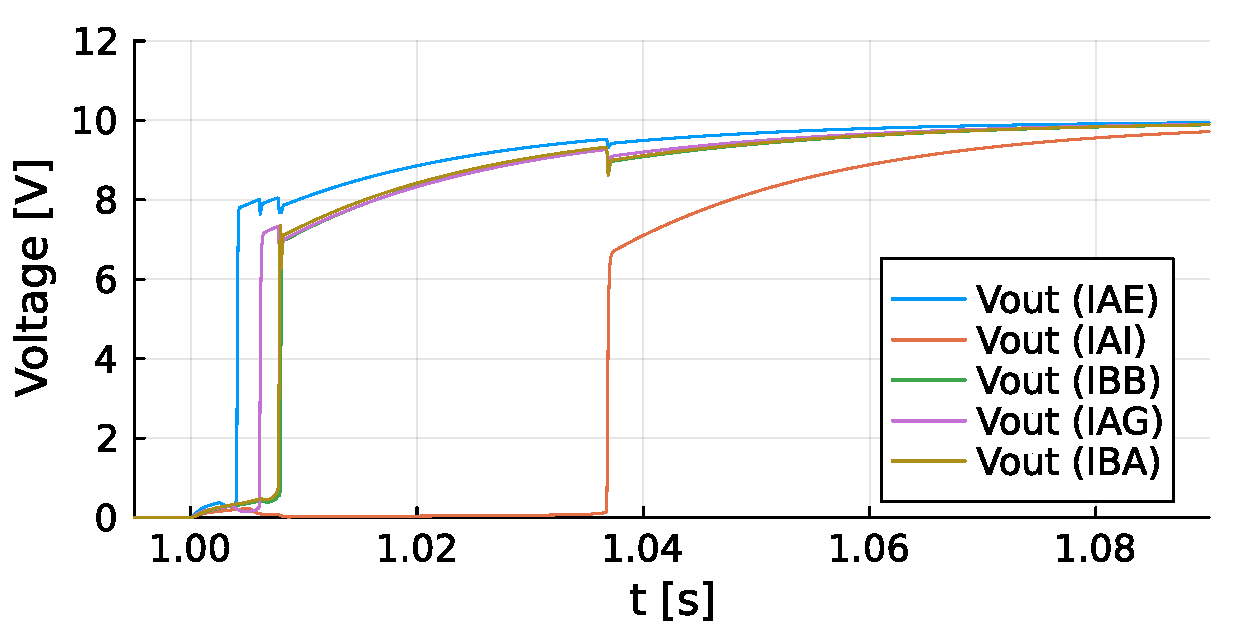
\includegraphics[height=.20\textheight]{acini_voltages_10.pdf}}%
  \hspace{1cm}
  \subfloat[][Acini currents]{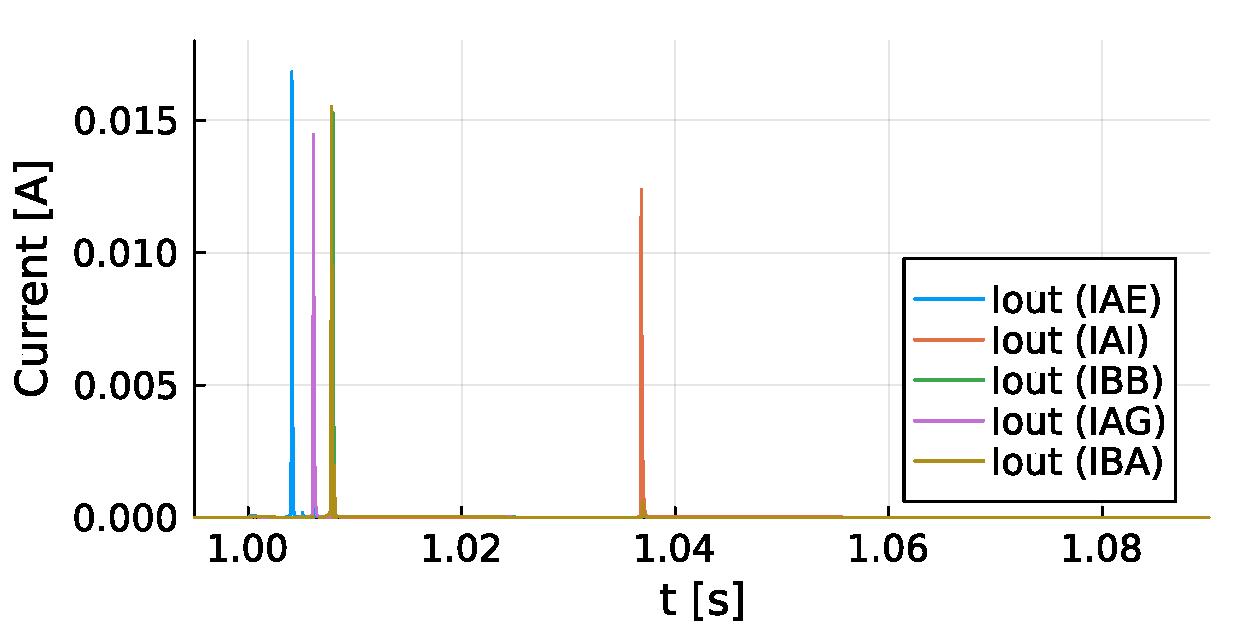
\includegraphics[height=.20\textheight]{acini_currents_10.pdf}}
  \caption{(Electrically equivalent) mechanical simulation for acini
    and aiways.  Step amplitude is 10V.}
  \label{fig:mechanical_results_10}
\end{figure}

% Test 1
%% Airways
\begin{table}[H]\centering
  {\renewcommand{\arraystretch}{1.2}
    \begin{tabularx}{\textwidth}{|P{6em}|C|C|C|C|}
      \hline
      \rowcolor{bluePoli!40}
      \textsc{Airways}
      & IAD
      & IAF
      & IAH
      & IBL\\
      \hline
      \rowcolor{yellow!40}$V_{\text{in,th}}$ [V]
      & 4.67
      & 4.99
      & 5.29
      & 5.59\\
      \hline
      \rowcolor{yellow!40}$T_{\text{open}}$ [s]
      & 1.00246
      & 1.00356
      & 1.00501
      & 1.00611\\
      \hline
      \rowcolor{orange!40}Activ. order
      & 1$^{\circ}$
      & 2$^{\circ}$
      & 4$^{\circ}$
      & 5$^{\circ}$\\
      \hline
    \end{tabularx}
  }
  \caption{Airways opening times values and total activation order
    when test \#1 is performed.}
  \label{tab:airways_test1}
\end{table}

%% Acini
\begin{table}[H]\centering
  {\renewcommand{\arraystretch}{1.2}
    \begin{tabularx}{\textwidth}{|P{6em}|C|C|C|C|C|}
      \hline
      \rowcolor{bluePoli!40}
      \textsc{Acini}
      & IAE
      & IAG
      & IAI
      & IBA
      & IBB\\
      \hline
      \rowcolor{yellow!40}$V_{\text{in,th}}$ [V]
      & 7.96
      & 8.69
      & 9.25
      & 6.79
      & 7.01\\
      \hline
      \rowcolor{yellow!40}$T_{\text{open}}$ [s]
      & 1.00411
      & 1.00616
      & 1.03686
      & 1.00781
      & 1.00796\\
      \hline
      \rowcolor{orange!40}Activ. order
      & 3$^{\circ}$
      & 6$^{\circ}$
      & 9$^{\circ}$
      & 7$^{\circ}$
      & 8$^{\circ}$\\
      \hline
    \end{tabularx}
  }
  \caption{Acini opening times values and total activation order
    when test \#1 is performed.}
  \label{tab:acini_test1}
\end{table}

The second test is providing a voltage capable of opening some of the
modules constituting the subtree.  Opening times and activation orders
are summarized into \Cref{tab:airways_test2,tab:acini_test2}.
Relative airway activation order is increasing from proximal to
distal.  Only distal acini are activated due to their lower diode
thresholds, the rest remains closed.

\begin{figure}[H]\centering
  \subfloat[][Airways voltages]{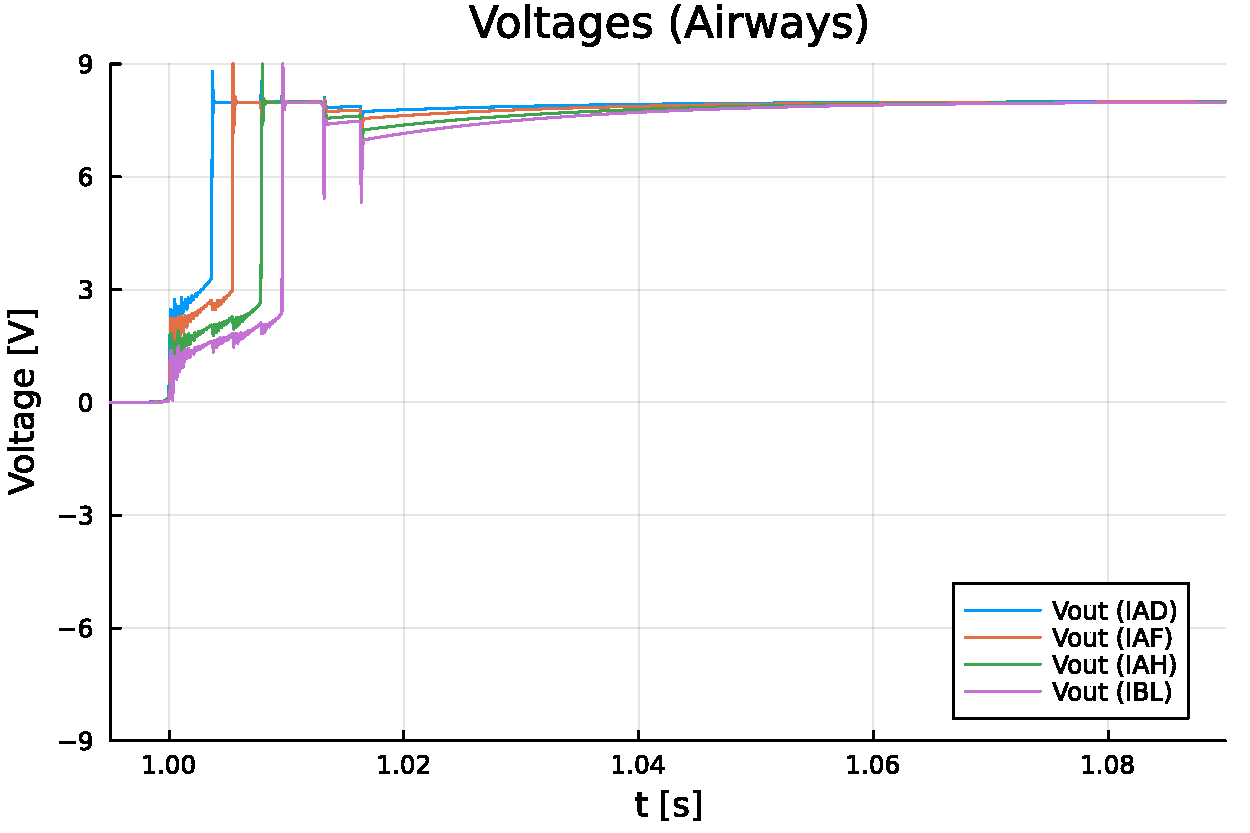
\includegraphics[height=.20\textheight]{airways_voltages_8.pdf}}%
  \hspace{1cm}
  \subfloat[][Airways currents]{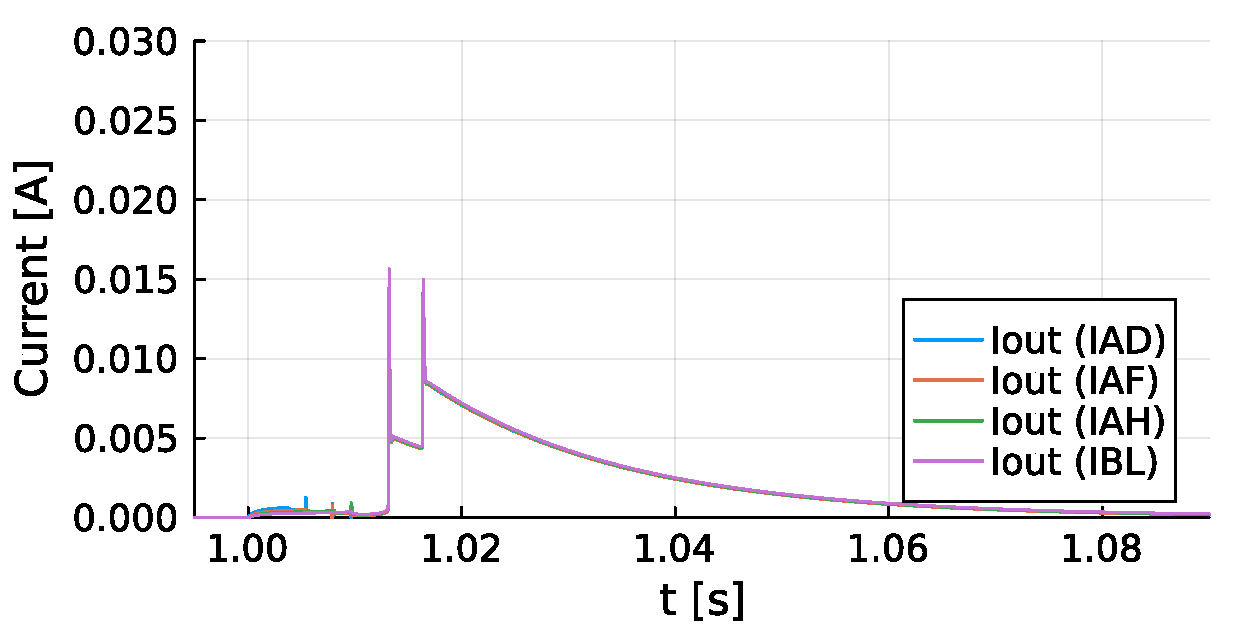
\includegraphics[height=.20\textheight]{airways_currents_8.pdf}}\\
  \subfloat[][Acini voltages]{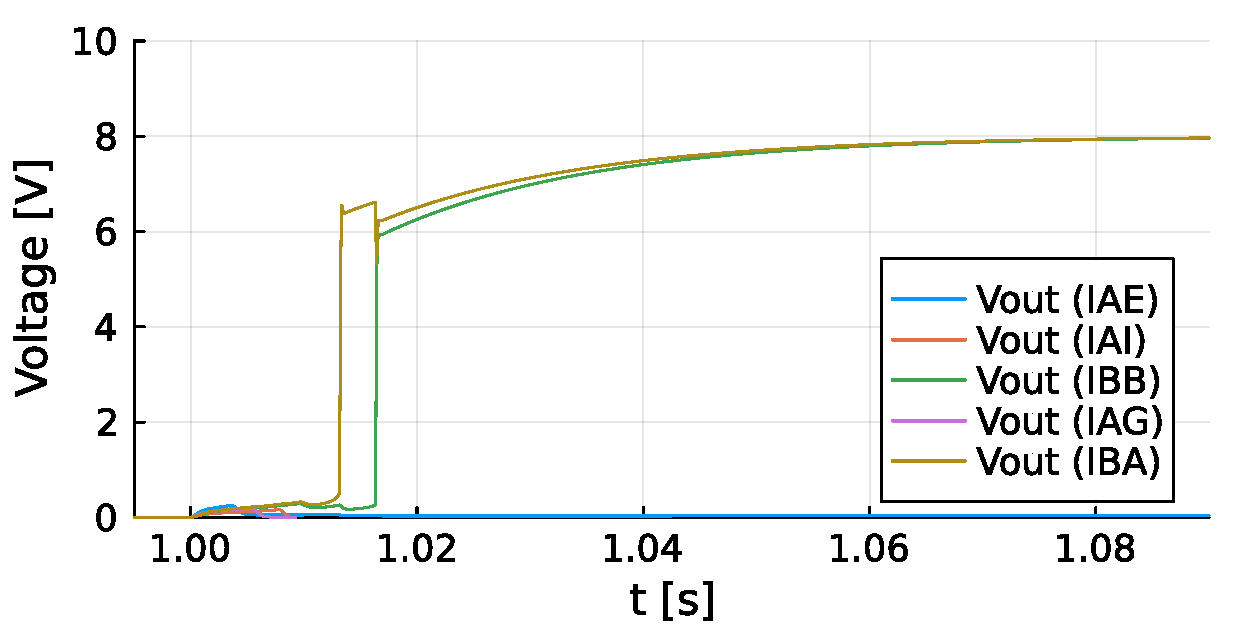
\includegraphics[height=.20\textheight]{acini_voltages_8.pdf}}%
  \hspace{1cm}
  \subfloat[][Acini currents]{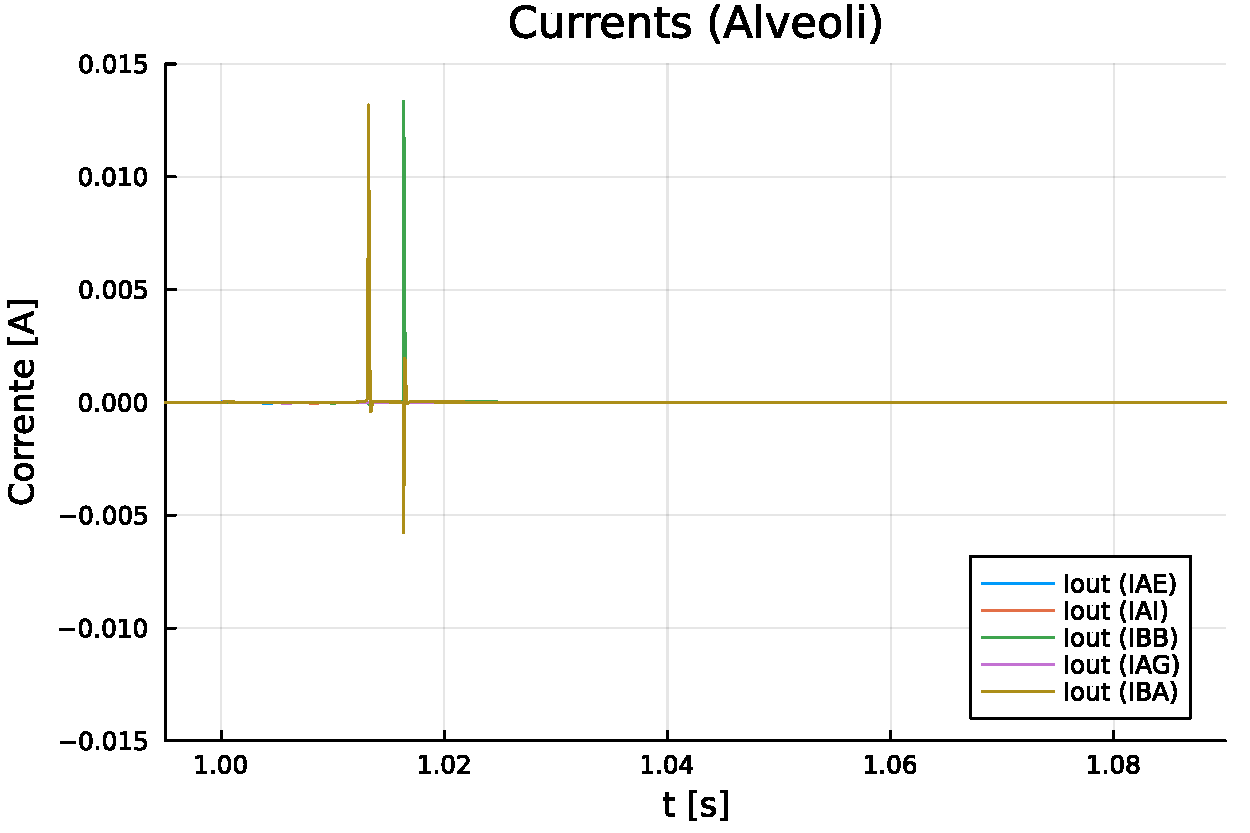
\includegraphics[height=.20\textheight]{acini_currents_8.pdf}}
  \caption{(Electrically equivalent) mechanical simulation for acini
    and aiways.  Step amplitude is 8V.}
  \label{fig:mechanical_results_8}
\end{figure}

% Test 2
%% Airways
\begin{table}[H]\centering
  {\renewcommand{\arraystretch}{1.2}
  \begin{tabularx}{\textwidth}{|P{6em}|C|C|C|C|}
    \hline
    \rowcolor{bluePoli!40}
    \textsc{Airways}
    & IAD
    & IAF
    & IAH
    & IBL\\
    \hline
    \rowcolor{yellow!40}$V_{\text{in,th}}$ [V]
    & 4.67
    & 4.99
    & 5.29
    & 5.59\\
    \hline
    \rowcolor{yellow!40}$T_{\text{open}}$ [s]
    & 1.00361
    & 1.00536
    & 1.00781
    & 1.00961\\
    \hline
    \rowcolor{orange!40}Activ. order
    & 1$^{\circ}$
    & 2$^{\circ}$
    & 3$^{\circ}$
    & 4$^{\circ}$\\
    \hline
  \end{tabularx}
}
\caption{Airways opening times values and total activation order when
  test \#2 is performed.}
\label{tab:airways_test2}
\end{table}

%% Acini
\begin{table}[H]\centering
  {\renewcommand{\arraystretch}{1.2}
    \begin{tabularx}{\textwidth}{|P{6em}|C|C|C|C|C|}
      \hline
      \rowcolor{bluePoli!40}
      \textsc{Acini}
      & IAE
      & IAG
      & IAI
      & IBA
      & IBB\\
      \hline
      \rowcolor{yellow!40}$V_{\text{in,th}}$ [V]
      & 7.96
      & 8.69
      & 9.25
      & 6.79
      & 7.01\\
      \hline
      \rowcolor{yellow!40}$T_{\text{open}}$ [s]
      & $+\infty$
      & $+\infty$
      & $+\infty$
      & 1.01316
      & 1.01636\\
      \hline
      \rowcolor{orange!40}Activ. order
      & ---
      & ---
      & ---
      & 5$^{\circ}$
      & 6$^{\circ}$\\
      \hline
    \end{tabularx}
    \caption{Acini opening times values and total activation order
      when test \#2 is performed.}
    \label{tab:acini_test2}
  }
\end{table}

%%% Local Variables:
%%% mode: LaTeX
%%% TeX-master: "../Thesis"
%%% End:
